\documentclass{beamer}
\usepackage[utf8]{inputenc}
\usepackage{xcolor}
\usepackage[T1]{fontenc}
\usepackage[normalem]{ulem}
\usetheme{Antibes}

\title{Projet Optimisation :\\Support Vector Machine}
\author{K. Kamtue \& Cl. Réda}
\institute{\textsc{ENS Cachan}}
\date{\today}

\setbeamerfont{page number in head/foot}{size=\large}
\setbeamertemplate{footline}[frame number]

\begin{document}
\maketitle
\tableofcontents
\setlength{\parindent}{1cm}

\section{Description du projet}

\subsection{Sujet}

\begin{frame}
\tableofcontents[currentsubsection]
\end{frame}

\begin{frame}
\frametitle{Sujet}
\framesubtitle{\emph{Support Machine Vector}}

\begin{center}
\textbf{Objectif :} Faire de l'apprentissage supervisé
\end{center}

\begin{itemize}
\item Appliqué à la classification binaire

         \begin{figure}
         \centering
         \caption{Exemple avec deux classes (rouge et noire)}
         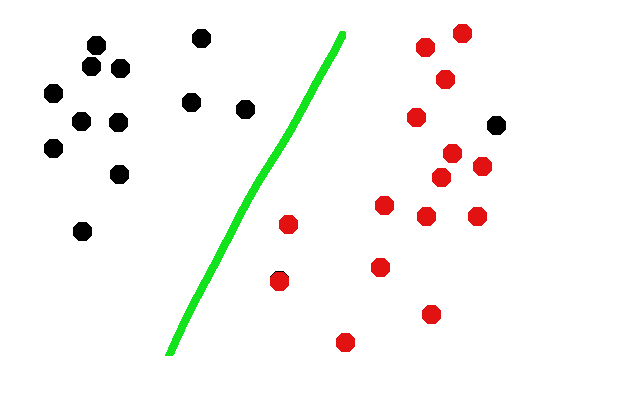
\includegraphics[scale=0.3]{images/voronoi.png}
         \end{figure}

\item Recherche d'une frontière linéaire $f : x \rightarrow \omega^Tx$ vérifiant (condition 1) :

         \begin{center}
         $\forall i, y_i = -1 \Rightarrow f(x_i) \leq -1$\\
         $\forall i, y_i = 1 \Rightarrow f(x_i) \geq 1$\\
         $\Leftrightarrow \forall i, y_i f(x_i) \geq 1$
         \end{center}
\end{itemize}

\end{frame}

\subsection{Le problème d'optimisation}

\begin{frame}
\frametitle{Le problème d'optimisation}
\framesubtitle{Recherche du problème d'optimisation}

\begin{block}{Naïvement}
$\gamma$ est la distance entre les droites $f(x) = 1$ et $f(x) = -1$.

      \begin{center}
        $max_{w}$ $\gamma = \frac{2}{\|w\|}$\\
        avec $\forall i, y_i f(x_i) \geq 1$\\

       \bigskip
        $\Leftrightarrow min_{w}$ $\|w\|$ \\
        avec $\forall i, y_i f(x_i) \geq 1$\\
       \bigskip
        $\Leftrightarrow min_{w}$ $\frac{1}{2} \|w\|^2$\\
        avec $\forall i, y_i f(x_i) \geq 1$\\
      \end{center}

\end{block}

\end{frame}

\begin{frame}
\frametitle{Le problème d'optimisation}
\framesubtitle{Amélioration}

\begin{block}{En rendant le problème toujours faisable}

Pénaliser les erreurs de classification avec les $(z_i)_i$ et $C$ :

           \begin{center}
           $min_{w}$ $\frac{1}{2} \|w\| + C \sum_{i \leq m}z_i$\\
           avec $\forall i, z_i \geq 0$\\
           $\forall i, y_i (\omega^{T} x_i) \geq 1 - z_i$\\
           \end{center}

\end{block}

\end{frame}

\subsection{Implémentation}

\begin{frame}
\tableofcontents[currentsubsection]
\end{frame}

\begin{frame}
\frametitle{Implémentation}
\framesubtitle{Résolution du problème d'optimisation}

\begin{itemize}
\item Utilisation de la méthode de Newton :

\begin{block}{Rappel : Mise à jour du vecteur $x$ avec la méthode de Newton}
          \begin{center}
          $x_{n+1} \leftarrow x_{n} + size \times \nabla^2 obj(x_n)^{-1}\nabla obj(x_n)$
          \end{center}

  (ici, en cherchant $size$ par \emph{backtracking line search})
\end{block}

\item Rendre le problème indépendant de la \emph{dimension} (\textbf{dépendant du nombre d'échantillons} !) en résolvant le \emph{problème dual};

\item Utiliser la méthode de la barrière logarithmique.

\end{itemize}

\end{frame}

\begin{frame}
\frametitle{Implémentation}
\framesubtitle{Le problème dual}

Après calcul du lagrangien, minimisation en $\omega$ et $z$ ($\lambda$ multiplicateur de Lagrange) :

\begin{block}{Problème dual}
             \begin{center}
             $max_{\lambda \in \mathbb{R}^{+m}} -\frac{1}{2}\|\sum_i\lambda_iy_ix_i\|^2_2 + $\textbf{1}$^T\lambda$\\ 
             avec $\forall i, 0 \leq \lambda_i \leq C$ si $z_i > 0$\\
             \end{center}
\end{block}

\begin{block}{Obtenir la solution du primal à partir de celle du dual}
             \begin{center}
               $\omega^{*} = \sum_i \lambda^{*}_i y_i x_i$
             \end{center}
\end{block}

\end{frame}

\begin{frame}
\frametitle{Implémentation}
\framesubtitle{Rendre le problème indépendant de la dimension}

Utilisation de l'\emph{astuce du noyau} :

\begin{block}{Problème dual}
Soit $K = X^TX$ (noyau). Alors :
                 \begin{center}
                 $max$ $-\frac{1}{2}\lambda^Tdiag(y)Kdiag(y)\lambda+$\textbf{1}$^T\lambda$\\
                 avec $\forall i, 0 \leq \lambda_i \leq C$ 
                 \end{center}
\end{block}

\end{frame}

\begin{frame}
\frametitle{Implémentation}
\framesubtitle{Supprimer les contraintes d'inégalité}

Utilisation de la \emph{méthode de la barrière logarithmique} :

\begin{block}{Fonction barrière pour éliminer les contraintes d'inégalité}
          \begin{center}
          $\Phi(\lambda) = \sum_i (- log(C - \lambda_i) - log(\lambda_i))$\\
          $= \sum_i log(\frac{1}{(C - \lambda_i)\lambda_i})$\\
          $= - \sum_i log((C - \lambda_i)\lambda_i)$ 
          \end{center}
\end{block}

\begin{block}{Problème d'optimisation final}
          \begin{center}
          $max$ $-\frac{1}{2}\lambda^Tdiag(y)Kdiag(y)\lambda+$\textbf{1}$^T\lambda + \Phi(\lambda)$\\ 
          \end{center}
\end{block}

\end{frame}

\section{Résultats}

\subsection{Détails de l'implémentation}

\begin{frame}
\tableofcontents[currentsubsection]
\end{frame}

\begin{frame}
\frametitle{Détails de l'implémentation}
\framesubtitle{Tracé de la convergence de la méthode de Newton}

         \begin{figure}
         \centering
         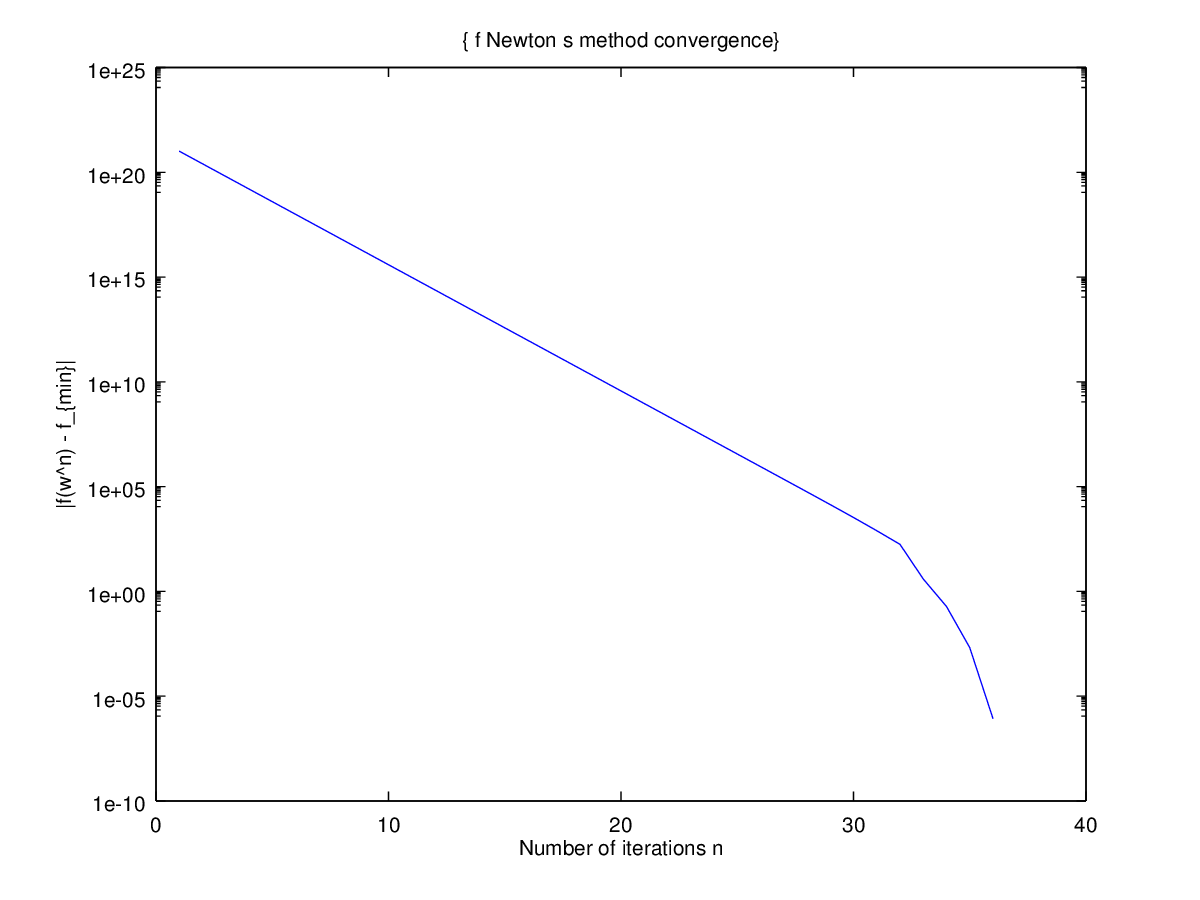
\includegraphics[scale=0.4]{images/cvnewton4.png}
         \end{figure}

\end{frame}

\begin{frame}
\frametitle{Détails de l'implémentation}
\framesubtitle{Dépendance en la taille de l'échantillon}

         \begin{figure}
         \centering
         \caption{Tableau récapitulatif}
         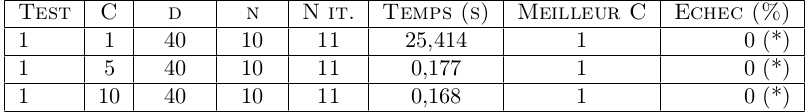
\includegraphics[scale=0.4]{images/tabl1.png}
         \end{figure}

\end{frame}

\begin{frame}
\frametitle{Détails de l'implémentation}
\framesubtitle{Accélération de la convergence quand $C$ augmente}

         \begin{figure}
         \centering
         \caption{Tableau récapitulatif}
         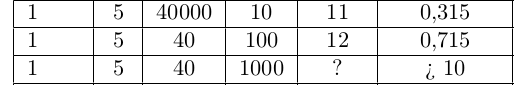
\includegraphics[scale=0.6]{images/tabl2.png}
         \end{figure}

\end{frame}

\subsection{Tracé de la frontière de classification}

\begin{frame}
\tableofcontents[currentsubsection]
\end{frame}

\begin{frame}
\frametitle{Tracé de la frontière de classification}
\framesubtitle{Pour $C = 5, n = 150, d = 200$}

Points centrés réduits avec des fonctions gaussiennes (2D) :

         \begin{figure}
         \centering
         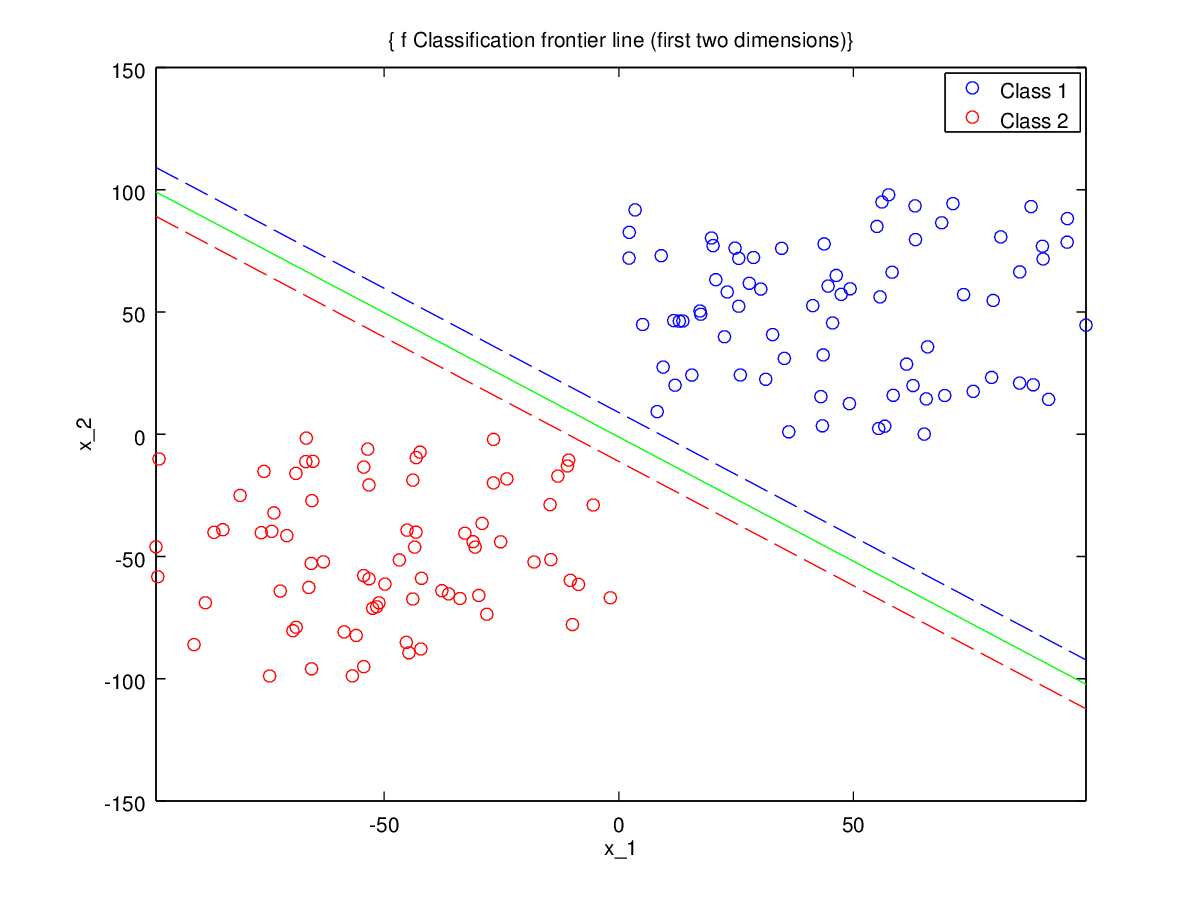
\includegraphics[scale=0.4]{images/line4.png}
         \end{figure}

\end{frame}

\begin{frame}
\frametitle{Tracé de la frontière de classification}
\framesubtitle{Pour $C = 5, n = 150, d = 200$}

Points centrés réduits avec des fonctions gaussiennes (3D) :

         \begin{figure}
         \centering
         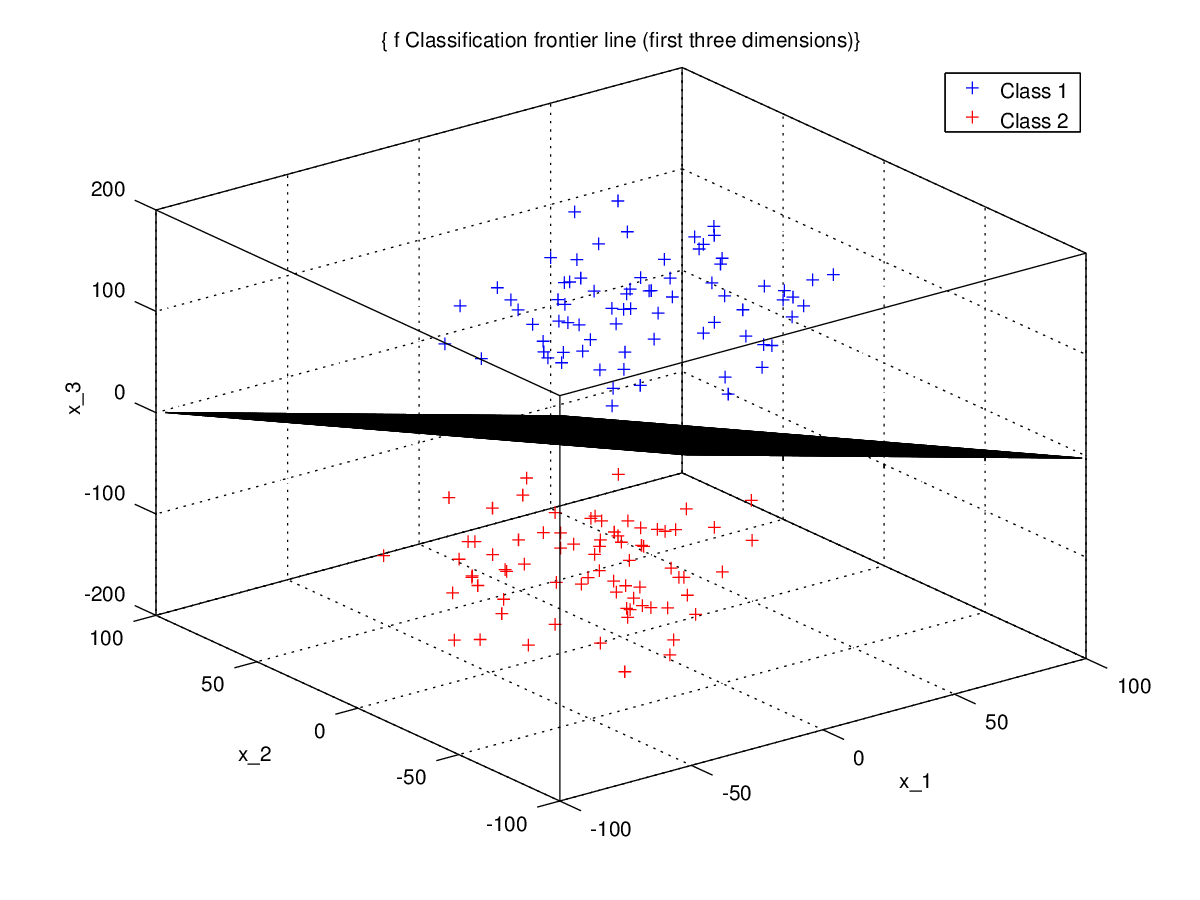
\includegraphics[scale=0.4]{images/plane4.png}
         \end{figure}

\end{frame}

\begin{frame}
\frametitle{Tracé de la frontière de classification}
\framesubtitle{Pour $C = 5, n = 150, d = 200$}

Génération avec des fonctions gaussiennes (2D) :

         \begin{figure}
         \centering
         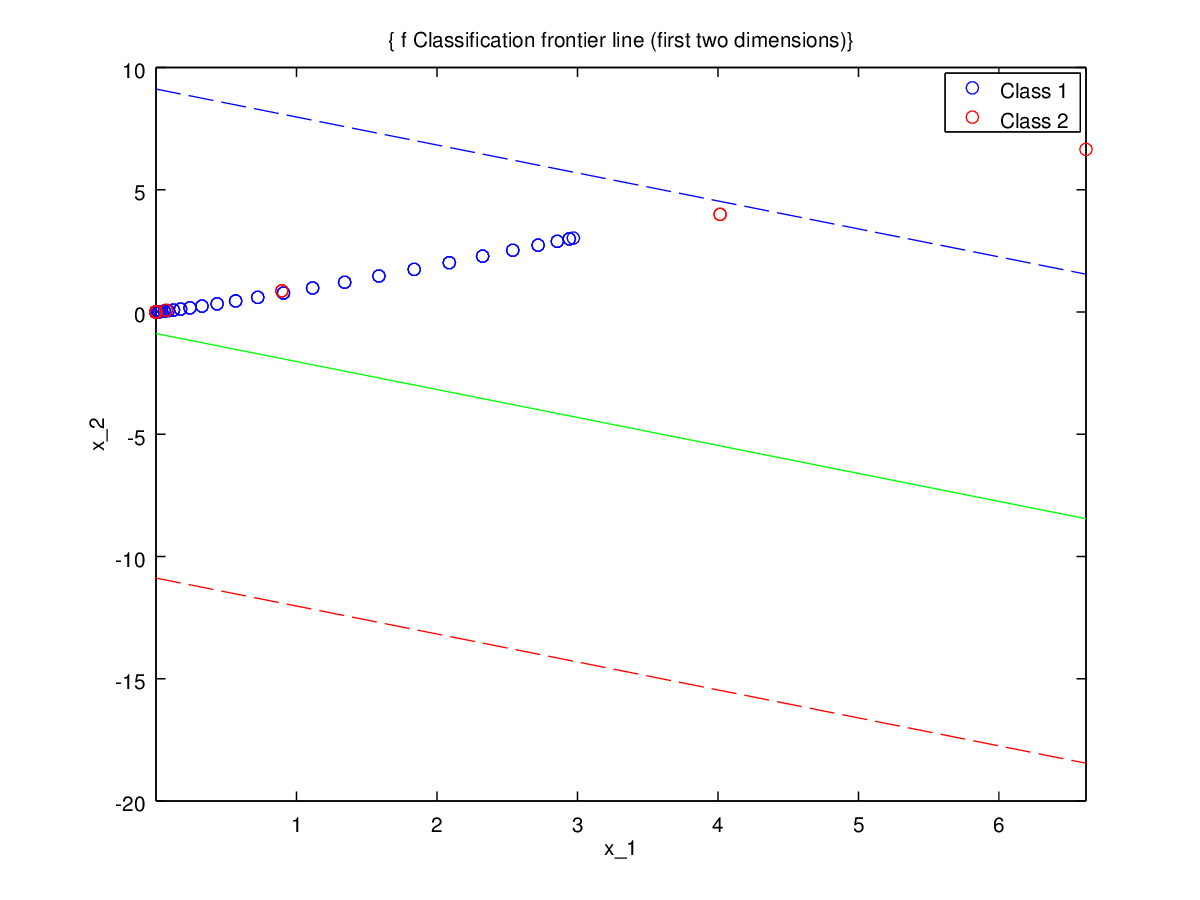
\includegraphics[scale=0.4]{images/line5.png}
         \end{figure}

\end{frame}

\begin{frame}
\frametitle{Tracé de la frontière de classification}
\framesubtitle{Pour $C = 5, n = 150, d = 200$}

Génération avec des fonctions gaussiennes (3D) :

         \begin{figure}
         \centering
         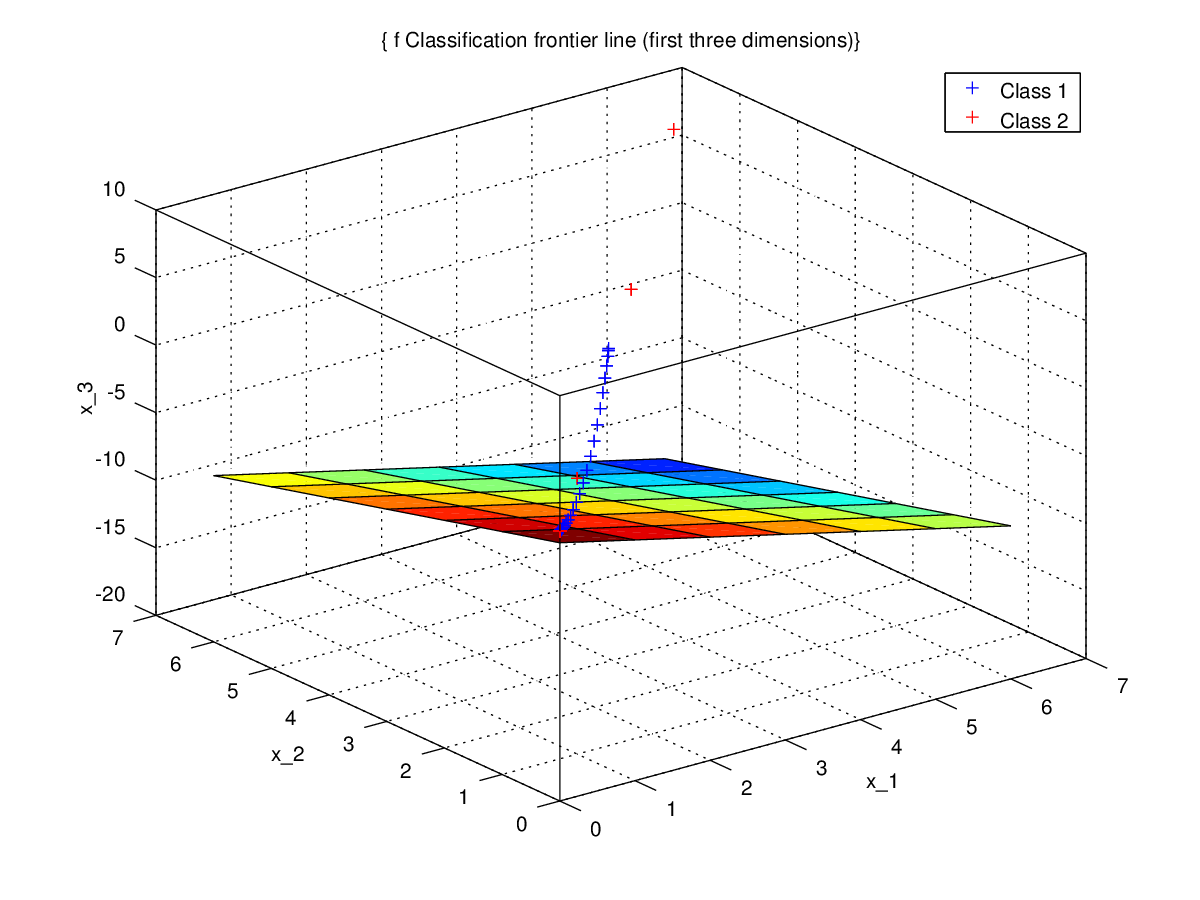
\includegraphics[scale=0.4]{images/plane5.png}
         \end{figure}

\end{frame}

% \section{Extensions}

% \begin{frame}
% \frametitle{Extensions}

% \begin{itemize}
% \item Validation croisée pour le choix de la meilleure valeur de C

% \item %TODO
% \end{itemize}

% \end{frame}

\end{document}
